\section{Moderne Enterprise-Architektur}

\begin{frame}{Event-Driven Architecture}
    \begin{itemize}
        \item Bisher: Expliziter Aufruf von Funktionalitäten
        \item Jetzt: Impliziter Aufruf durch Reaktion auf Ereignisse \cite{garlanShawImplizit}
        \item System reagiert asynchron auf Zustandsänderung (Ereignis in System)
        \item Alte Idee: David Garlan und Mary Shaw, 1994, \textit{An Introduction to Software Architecture}
    \end{itemize}
\end{frame}

\begin{frame}{Event-Driven Architecture: Komponenten}
    \begin{itemize}
        \item Event: Kapselt Information einer Zustandsänderung eines Systems \cite{eda}
        \item Produzent: Erzeugt Event
        \item Publisher: Publiziert erzeugtes Event
        \item Konsument: Reagiert auf Event
        \item Mediator: Vermittler zwischen Produzenten und Konsumenten
        \item Event-Broker: Infrastruktur für Gesamtheit der Vermittler
    \end{itemize}
\end{frame}

\begin{frame}{Event-Driven Architecture: Struktur}
    \begin{figure}[!h]
        \centering
        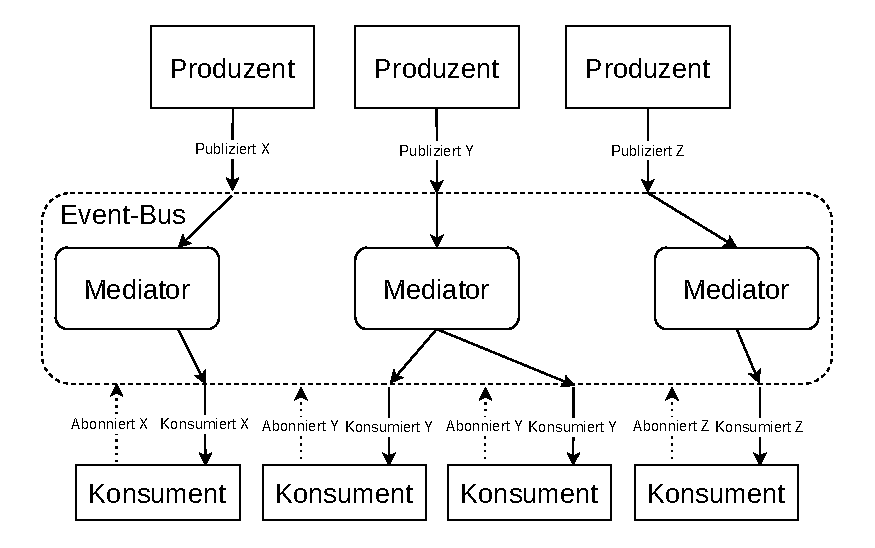
\includegraphics[scale=0.55]{imglib/eda/eda.drawio}
        \caption{Vertrag zwischen Produzenten und Konsumenten am Event-Bus}
        \label{fig:eda}
    \end{figure}
\end{frame}

\begin{frame}{Event-Driven Architecture: Beispiel E-Commerce I}
    \begin{itemize}
        \item \texttt{OrderCreated}: Genau dann, wenn Bestellung aufgegeben wird
        \item \texttt{PaymentProcessed}: Genau dann, wenn Bezahlvorgang abgeschlossen wird
        \item \texttt{ShipmentInitiated}: Genau dann, wenn Bestellung versandt wird
        \item Event-Kette: $ \texttt{OrderCreated} \rightarrow \texttt{PaymentProcessed} \rightarrow \texttt{ShipmentInitiated}$
        \item Implementierung in Diensten: OrderService, PaymentService, ShipmentService
    \end{itemize}
\end{frame}

\begin{frame}{Event-Driven Architecture: Beispiel E-Commerce II}
    \begin{figure}[!h]
        \centering
        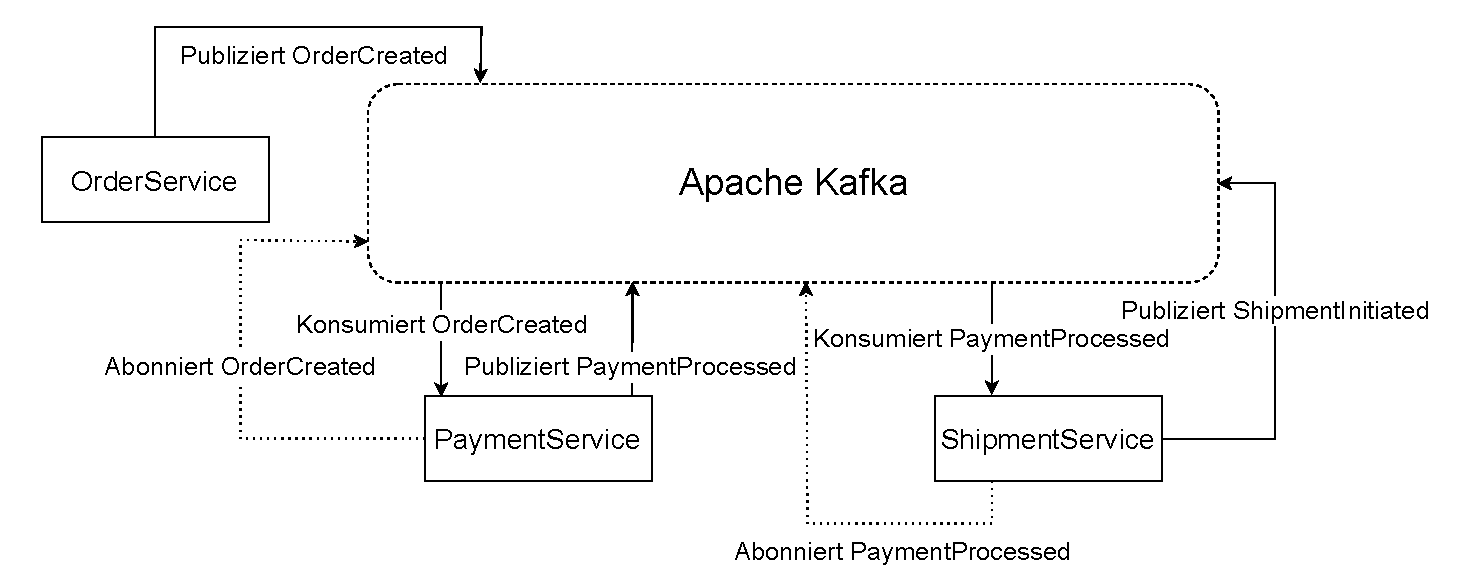
\includegraphics[scale=0.5]{imglib/eda/eda-ecommerce.drawio}
        \caption{E-Commerce-Beispiel mit Event-Driven Architecture}
        \label{fig:edaecommerce}
    \end{figure}
\end{frame}

\begin{frame}{Event-Driven Architecture: Agilität}
    \begin{itemize}
        \item Event ist Vertrag zwischen Produzent und Konsument am Event-Broker\\
        $\rightarrow$ Hohe Kohäsion $\rightarrow$ Lose Kopplung
        \item Feature: Menge von Events, deren Produzenten und Konsumenten\\
        $\rightarrow$ Klare Abgrenzung $\rightarrow$ einfach definierbare Iterationen
        \item Events sind sehr realitätsnah - domain-driven
        \item Sehr hohe Flexibilität \& maximale Skalierung durch lose Kopplung
        \item Schnelle Auslieferung, kurze Intervalle
        \item Exzellente Kombination mit Microservices \& Cloud-Integration
        \item Aber: Erhöhte Komplexität $\rightarrow$ Hohe Anforderungen an Entwickler
    \end{itemize}
\end{frame}